\chapter{Обзор литературы}
\section{Вариабельность сердечного ритма }

Вариабельность сердечного ритма (Heart rate variability, HRV) это явление изменения частоты сердечного ритма.

Вариабельность сердечного ритма сильно зависит от эмоционального \cite{hrv_and_sensitivity, hrv_and_respiratory} и физического \cite{hrv_and_phisical_health} здоровья человека и может использоваться как его показатель.

Существуют два основных причины колебания частоты сердечного ритма \cite{two_rates_hrv}.

\begin{itemize}
	\item Колебания, вызванные дыхательной аритмией. При этом частота сердечных сокращений изменяется в связи с дыханием и можно отследить частоту дыхания.
	\item Низкочастотные колебания артериального давления. Это явление называется волнами Майера \cite{mayer_wave} артериального давления и, как правило, имеют частоты порядка 0,1 Гц.
\end{itemize}

Для наблюдения за сердечным ритмом применяются следующие методы:

\begin{itemize}
	\item ЭКГ (электрокардиография) \cite{EKG};
	\item баллистокардиография  \cite{Ballistocardiograms};
	\item фотоплетизмография \cite{Photoplethysmography}.
\end{itemize}

ЭКГ считается методом, дающим наиболее четкий сигнал.


\subsection{Общие принципы функционирования сердца}

Выталкивание крови из сердца каждую минуту - это важнейшее сердечно-сосудистое событие, необходимое для поддержания циркуляции крови по всему телу. Сердце, помимо объема циркулирующей крови и силы мыщечных сокращений, должно выдерживать цикличность расслабления и сжатия, для выполнения своей функциональности. Эта закономерность основана на серии сложных электрофизиологических явлений в тканях сердца, которые можно контролировать, используя устройство, называемое электрокардиограф.
 
Событиями необходимыми для нормального сердечного цикла являются ритмические сокращения и расслабления мыщц предсердий и желудочков. Сердце состоит из 2 основных типов клеток: рабочих клеток и специализированных проводящих клеток. Рабочая клетки - это мышцы или миокард предсердий и желудочков. Из специализированных клетки  состоят синусоидально-предсердный (SA) узел, атриовентрикулярный (AB) узел, пучок Гиса и волокон Пуркинье (рис. \ref{ris:heart1}) \cite{heart_stracture}.
\begin{figure}[h]
	\begin{center}
		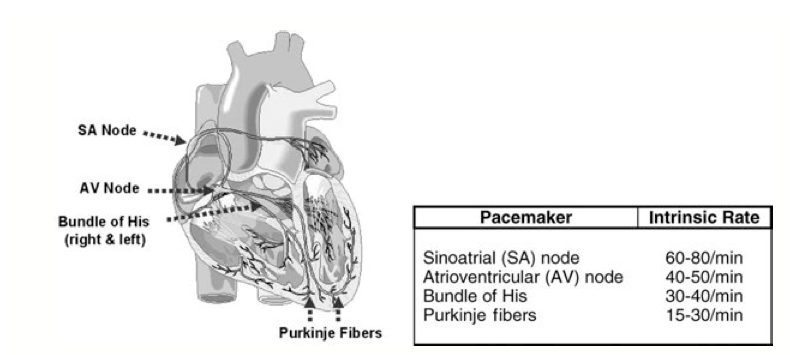
\includegraphics[scale = 0.6]{heart1}
		\caption{Строение сердца}
		\label{ris:heart1}
	\end{center}
\end{figure}

Специализированные клетки инициируют и проводят электрические импульсы по всему миокарду, и это регулирует ритм сердечного цикла. Для того, чтобы инициировать импульсы, специализированные клетки имеют свойство автоматизма, которое объясняет способность спонтанно инициировать электрические импульсы. Это свойство не зависит от нервов или гормонов, но реальная частота работы данных клеток может меняться под влиянием вегетативной нервной системы.

Каждый сердечный цикл начинается с импульса, спонтанно генерируемые узлом SA. Импульс впоследствии распространяется по всей оставшейся части проводящей соединительные ткани, на мышцы (миокард) клеток. Нарушения в этой системе генерации электрических импульсов (случайная генерация импульсов) называется аритмией.

\subsection{Электрофизиологические аспекты работы сердца}

Чтобы в полной мере понимать информацию и электрические импулься, описываемые ЭКГ, мы должны сначала рассмотреть основные понятия, касающиеся электрических потенциалов мембраной ткани сердца. Все клетки сердечной мембраны имеют заряженые положительно наружные поверхности из-за относительного распределения катионов. Этот мембранный потенциал покоя поддерживается с помощью активного транспортирующего механизма, называемого натрий-кальциевым насосом. Когда клетка стимулируется, ионные каналы открываются, обеспечивая приток ионов натрия и(/или) кальция, и тем самым, уходя из состояния потенциала покоя. Этот период деполяризации очень короткий, поскольку натриевые каналы резко закрываются, прекращая дальнейший приток натрия. Одновременно с этим калиевые каналы открыты и позволяют внутриклеточному калию диффундировать наружу, в то время как ионы натрия активно выкачиваются. Это восстанавливает положительный заряд снаружи мембраны, происходит процесс реполяризации, что возвращает мембрану к ее потенциалу покоя. Процессы деполяризации и реполяризации в целом называют потенциалом действия. Это процесс самостоятельно распосраняет импульс вдоль всей поверхности сердца и из одной клетки в другую, при условии, что их мембраны соединяются. (рис. \ref{ris:depolarization}) 

\begin{figure}[h]
	\begin{center}
		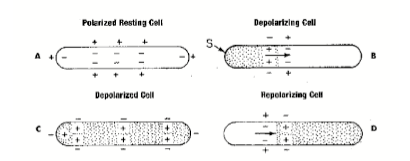
\includegraphics[scale = 1]{depolarization}
		\caption{Деполяризации и реполяризации клеточных мембран.
			A) покой, клеточной мембраны заряжена положительно по
			снаружи и отрицательно внутри. B) следующим стимулом
			(S) положительные ионы попадают в клетки, обращая эти полярности. C)
			Этот процесс продолжается до тех пор, пока вся клетка не является деполяризованной. D)
			Ионы возвращаются в их нормальное расположение и ячейки реполярицуется в потенциал покоя.}
		\label{ris:depolarization}
	\end{center}
\end{figure}

Все человеческие клетки демонстрируют это явление, но его назначение колеблется в зависимости от функции клетки. Цель потенциалов действия в нейронах инициировать высвобождение нейромедиаторов (нейромедиаторы - биологически активные химические вещества, посредством которых осуществляется передача электрохимического импульса от нервной клетки через синаптическое пространство между нейронами, а также, например, от нейронов к мышечной ткани или железистым клеткам.), которые либо возбуждают либо стабилизируют клеточные мембраны тканей. В скелете и сердечных мышцах клетки, активный потенциал которых сохраняет запасенный кальций, инициируют собственно сократительный процесс.

Клетки включенные в проводящую систему сердца являются уникальными в 2 аспектах. Как было сказано выше, они обладают свойством автоматизма. Физиологическое объяснение этого свойства заключается в частичной проницаемости мембраны в состоянии потенциала покоя для кальция и/или ионов натрия. Постепенная внутренняя ‘утечка’ катионов уменьшает напряжение потенциала покоя до тех пор, пока не будет достигнут порог. На этот момент, все каналы будут открыты и быстрый приток катионов деполяризует мембраны.

Второй уникальной особенностью этой специализированной ткани является тот факт, что в отличие от классических нервной ткани, эти клетки не высвобождают нейромедиаторы. Вместо этого, они находятся в непосредственном контакте с сердечной мышцы, и их потенциал действия инициирует деполяризацию клеток сердечной мышцы напрямую.
Клетки сердечной мышцы соединены друг с другом с помощью специальных приспособлений, называемых вставочными дисками. Это позволяет им функционировать как сплошной лист из клеток синцития. Синцитий в предсердиях отделен от желудочков слоем соединительной ткани, которая выступает в качестве изолятора. SA узел инициирует деполяризацию мышц предсердий, но слой изоляции исключает возможность распространение импулься на желудочки за исключением только одного места - узла AV. 

Атриовентрикулярный узел  задерживает и, наконец, транслирует импульс вдоль общего пучка волокон Гиса, который проникает в соединительную ткань, чтобы потом войти в желудочки. Импульс продолжается вдоль пучка и его ветвей, пока он, наконец, не достигает волокон Пуркинье, которые возбуждают синцитий желудочковой мышцы .

Потенциал действия отдельной клетки можно измерять, только используя микрозонды, вводимые через клеточную мембрану. 
Это слишком маленькое электрическое событие, чтобы оно могло быть измерено с помощью поверхностных электродов. Однако, потенциалы действия, которые распространяются по всему слою синцитиев сердца достаточно велики для того, чтобы быть замечены поверхностными электродами для процедуры записи, известной как ЭКГ. Важно понимать, что ЭКГ не может записывать напрямую электрические события, создаваемые специализированными клетками проводящей системы; их напряжение слишком мало. То, что вы наблюдаете на электрокардиограмме - это потенциалы действия в предсердных и желудочковых мышечных клетках. Однако, другие события также могут быть предсказаны исходя из кардиограммы.

\subsection{Методика записи ЭКГ}

Последовательность электрических импульсов сердечного цикла инициируется с помощью синусно-предсердного узла, так называемого ритмоводителя сердца. Это потому, что узел SA имеет более быстрый темп спонтанной генерации импульсов, чем остальные клетки специализированной ткани. Однако, если этот темп уменьшается, другие части этой специализированной системы могут получить контроль над темпом генерации импульсов.

Базовая линия ЭКГ называется изоэлектрической линии и обозначает состояние покоя потенциала мембраны. Отклонения от этой линии обозначается буквами в алфавитном порядке, и после каждого, линия при записи ЭКГ обычно возвращается к изоэлектрической. Первое отклонение - P-подъем, он отражает деполяризацию мышц клеток предсердий. Она не отражают сокращение этой мышцы, а также не отражают возбуждение из SA-узла. Об этих событиях делаются предположения на основе формы и последовательности P-подъема. 

\begin{figure}[h!]
	\begin{center}
		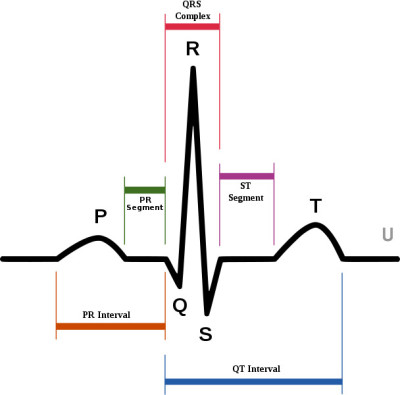
\includegraphics[scale=0.7]{QRS_for_features}
		\caption{Вид ЭКГ во время сокращения мыщц сердца}
		\label{ris:QRS}
	\end{center}
\end{figure}

Предполагается, что SA-узел генерирует импульс в начале Р-волны, и что сокращения предсердий начинается на пике Р-волны. Хотя за реполяризацией предсердий следует деполяризации, ЭКГ не дает никаких доказательств этого события. Популярным заблуждением является то, что изображение реполяризации скрыто под последующим QRS-комплексом.Однако, если это верно, реполяризация будет наблюдаться в тех случаях, когда комплекс QRS-комплекс задержан или отсутствует, например, в случае AV-блокады. Что не так. Правильное объяснение заключается в том, что реполяризация предсердий  слишком незначительная по амплитуде создаваемого электрического потенциала и не может быть записана с помощью поверхностных электродов.

QRS-комплекс отражает деполяризацию клеток мыщц желудочков. Интервал Q является первоначальным прогибом вниз, пик R - прогиб вверх, а S - это возвращение к базовой линии, или так называемой изоэлектрической точке. Часто, прогиб Q, увы, не видно и деполяризации представлена только как ‘RS’ комплекс. В любом случае, комплекс не
представляет собой сокращения желудочков. Предполагается, что сокращение начнется на пике R. В отличие от сокращения предсердий, сокращения желудочков могут быть увидены клинически с помощью прощупывания пульса специальными приспособлениями.

Больной с сердечным приступом может иметь нормальный QRS-комплекс на ЭКГ; мышечные клетки желудочков сердца деполяризуются, но там нет сокращения. Это явление называется электрической активностью без пульса. После деполяризации, мышцы желудочков реполяризуются, и этот процесс может достигать достаточно большой амплитуды, чтобы генерировать волны T на ЭКГ. 

PR интервал измеряется от начала зубца P до начала R пика. (Так часто делают, поскольку интервал Q часто неразличим.) Так как интервал PR начинается с деполяризации клеток мышц предсердий и заканчивается с началом деполяризации желудочков, можно предположить, что электрический импульс проходит через узел AV в желудочек во время этого интервала. Если интервал PR затягивается, можно сделать вывод, что AV блок присутствует.

\subsubsection{Немного об реализации записи ЭКГ}

В 1901 году голландский физиолог Виллем Эйнтховен разработал гальванометр, который мог бы записать электрическую активность сердца. Он обнаружил, что запись может быть произведена, как разница потенциалов действия  тока распространяющегося между отриьно и положительно заряженных электродов. (Третий электрод служит для заземления тока.) Он обнаружил, что записи варьируются в зависимости от расположения положительного и отрицательного электродов, и впоследствии описал тремя углами в виде треугольника с сердцем в середине. Эта конструкция известна сегодня как треугольника Эйнтховена, а 3 метода наложения электродов - известны как основные отведения от конечностей I, II и III (Рис. \ref{ris:3mainline}).

\begin{figure}[h!]	
	\begin{center}
		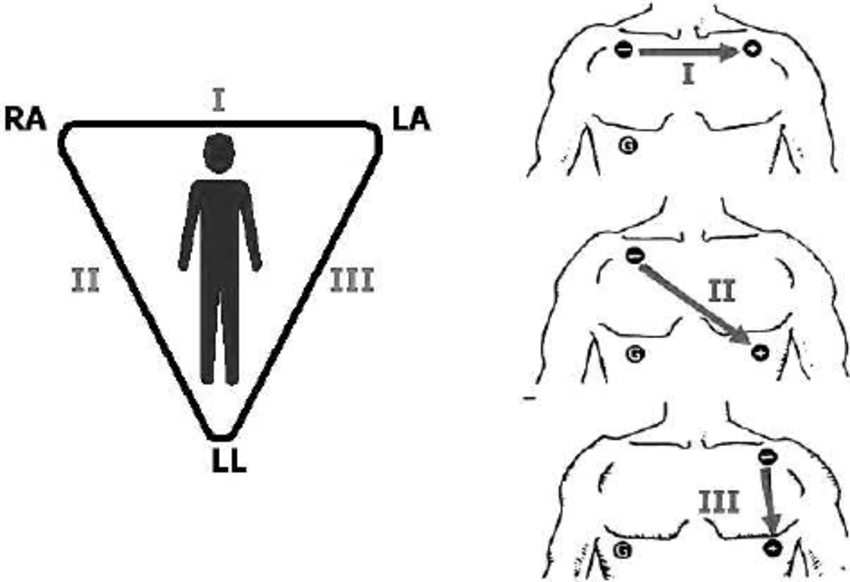
\includegraphics[scale = 0.3]{3mainline}
		\caption{схема трех основных отведений}
		\label{ris:3mainline}
	\end{center}
\end{figure}

Исследования продолжались на протяжении 20-го века, и дополнительно обнаружили, что электрические импульсы распространяются во многих направлениях через сердце. Сегодня кардиолог анализирует ЭКГ в 12 отведениях для помощи в диагностике инфаркта, гипертрофии и сложных аритмий.


\subsubsection{Резюмируя сказанное выше}

Повторим основную информацию о сердце.
Сердце обладает рядом свойств.

\begin{itemize}
	\item Свойство автоматизма - это способность сердца вырабатывать электрические импульсы при отсутствии внешних раздражений.
	\item Свойство проводимости - это способность к проведению возбуждения специальными клетками проводящей системы сердца и сократительного миокарда.
	\item Свойство возбудимости – это способность клеток проводящей системы сердца и сократительного миокарда возбуждаться под влиянием внешних электрических импульсов.
\end{itemize}

Возбуждение сердечной мышцы сопровождается возникновением изменяющейся разности потенциалов между наружной и внутренней поверхностью клеточной мембраны сердца.

При распространении по сердцу волны деполяризации наружная поверхность клетки приобретает отрицательный заряд, а во время реполяризации – положительный. Согласно концепции В. Эйнтховена, сердце в каждый момент сердечного цикла можно рассматривать как точечный единый диполь, который создает в окружающей его среде электрическое поле. Положительный полюс диполя (+) всегда обращен в сторону невозбужденного, а отрицательный полюс (–) – в сторону возбужденного участка сердца(рис. \ref{ris:dipol}).

\begin{figure}[h!]
	\begin{center}
		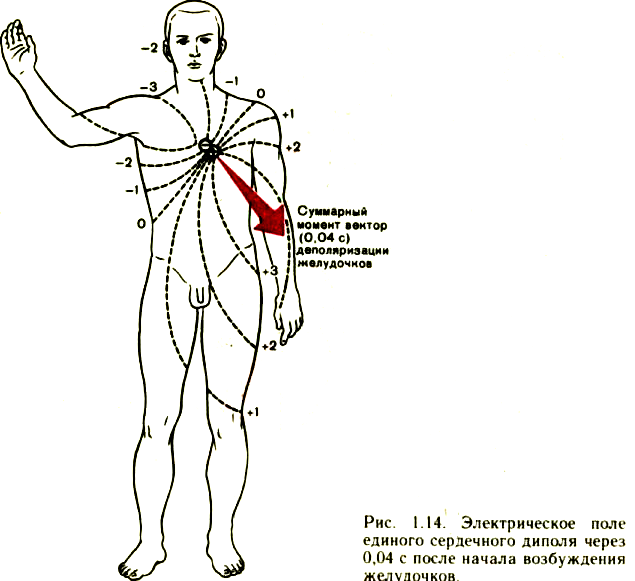
\includegraphics{heart-dipol}
		\caption{Поле сердечного диполя в отведениях}
		\label{ris:dipol}
	\end{center}
\end{figure}


Помещая положительный и отрицательный электроды в любые точки электрического поля, можно зарегистрировать разность потенциалов, существующую между этими точками в каждый момент деполяризации и реполяризации сердца. Конфигурация такой ЭКГ прежде всего будет зависеть от направления вектора диполя по отношению к электродам.

В настоящее время в клинической практике наиболее широко используют 12 отведений ЭКГ, запись которых является обязательной при каждом электрокардиографическом обследовании больного: 3 стандартных отведения, 3 усиленных однополюсных отведения от конечностей и 6 грудных отведений.

Стандартные отведения от конечностей регистрируют при следующем попарном подключении электродов:

\begin{itemize}
	\item I отведение – левая рука (+) и правая рука (–);
	\item II отведение – левая нога (+) и правая рука (–);
	\item III отведение – левая нога (+) и левая рука (–).
\end{itemize}

\subsection{Электрокардиограмма}



Электрокардиограмма – это запись колебаний разности потенциалов, возникающих на поверхности возбудимой ткани или в окружающей сердце проводящей среде при распространении волны возбуждения по сердцу.\cite{ekg1} Запись ЭКГ производится с помощью электрокардиографов и различных систем отведений ЭКГ. Каждое отведение регистрирует разность потенциалов, существующую между двумя определенными точками электрического поля сердца, в которых установлены электроды. Пример ЭКГ можно увидеть на рис. \ref{ris:RR}.

\begin{figure}[h!]
	\begin{center}
		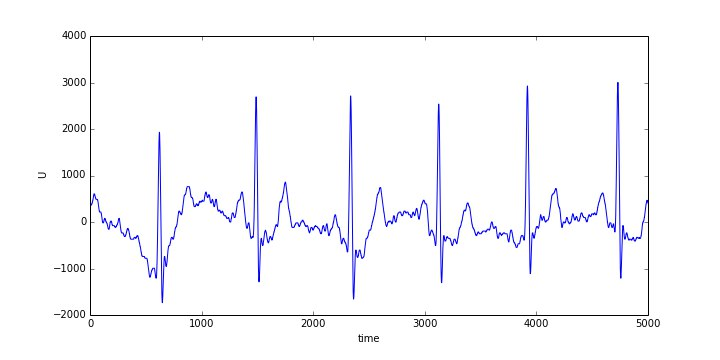
\includegraphics[scale=0.5]{real_ekg}
		\caption{ЭКГ}
		\label{ris:RR}
	\end{center}
\end{figure}

\subsection{RR}

Если рассматривать момент сокращения сердца более подробно \cite{polarization_heart} виден QRS-комплекс - изменения электрического потенциала, предшествующее сокращению сердца. За электрической активацией клеток (деполяризацией) следует механическое сокращение. Процесс сокращения сердечных мыщц состоит из следующих стадий (рис.\ref{ris:EKG}).

\begin{figure}[h!]
	\begin{center}
		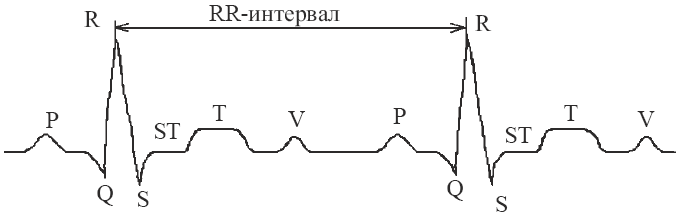
\includegraphics[scale = 0.7]{RR.png}
		\caption{EKG}
		\label{ris:EKG}
	\end{center}
\end{figure}

\begin{itemize}
	\item деполяризация предсердий; зубец P
	\item передача импульса желудочкам; интервал PR
	\item деполяризация желудочков; зубец R
	\item реполярицазия желудочков; зубец T
	\item мнения исследователей относительно причин происхождения зубца V различны.
\end{itemize}

Для различных отведений вид QRS комплекс может отличаться. Вместо пика R может быть глубокий минимум. Минимумы Q, S могут отсутствовать. Приведенный на рисунке выше пример соответствуют первому отведению.

По длительности интервалов, глубине минимумов и высоте максимумов врачи предсказывают различные характеристики и болезни.

RR-интервалом называется промежуток времени между R пиками (последовательными ударами сердца).


Нормально частотой серцебиения считается 60-100 ударов в минуту в состоянии покоя. Ниже приведены примеры RR-сигнала (последовательность RR-интервалов) (рис. \ref{ris:real_RR}).

\begin{figure}[h!]
	\begin{minipage}[h]{0.47\linewidth}
		\center{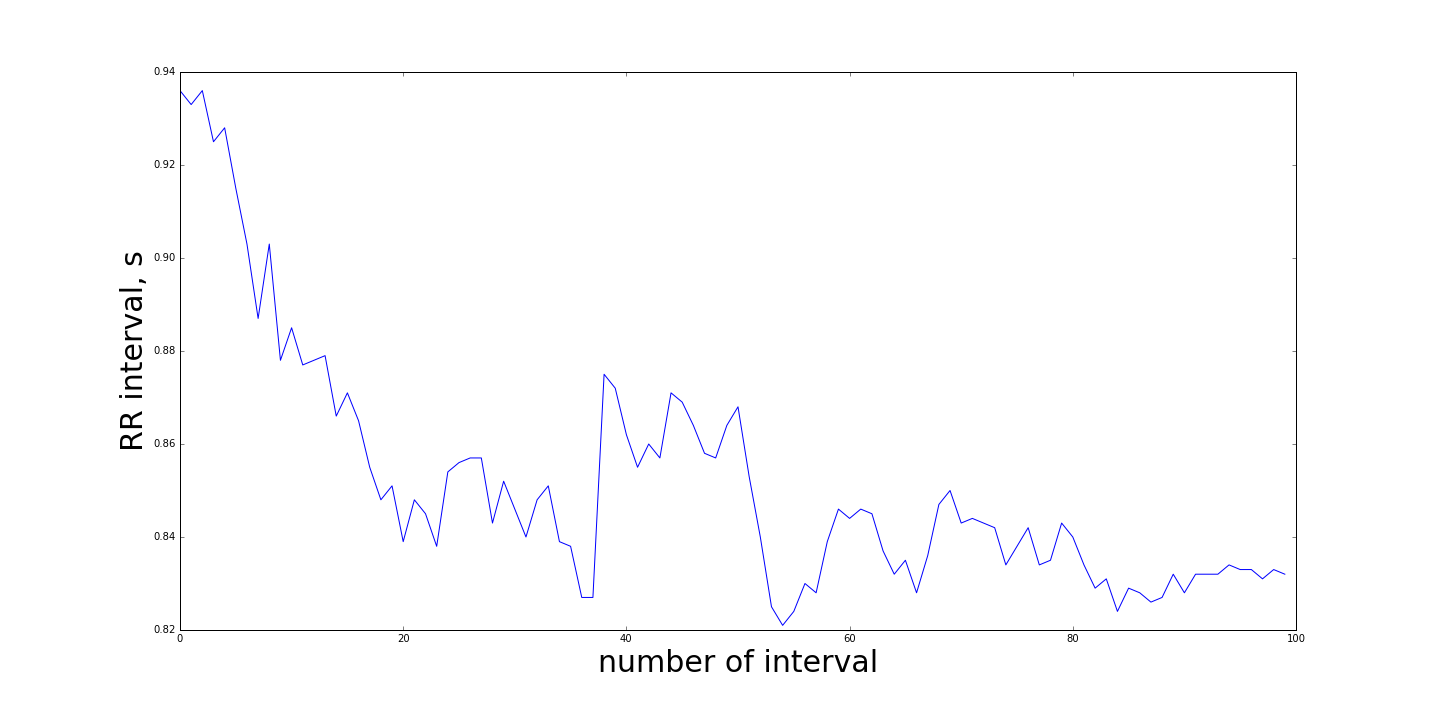
\includegraphics[width=1\linewidth]{rr_100}} a) \\
	\end{minipage}
	\hfill
	\begin{minipage}[h]{0.47\linewidth}
		\center{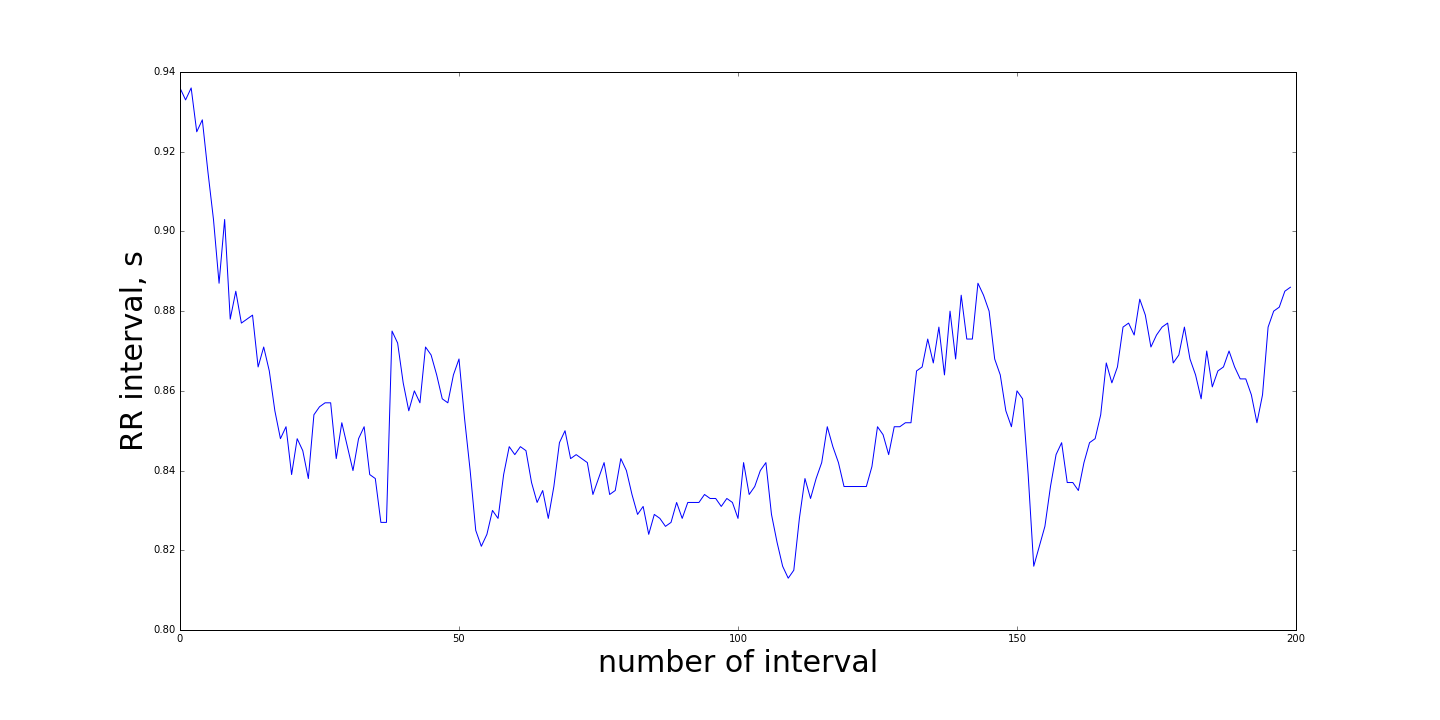
\includegraphics[width=1\linewidth]{rr_200}} \\b)
	\end{minipage}
	\vfill
	\begin{minipage}[h]{0.47\linewidth}
		\center{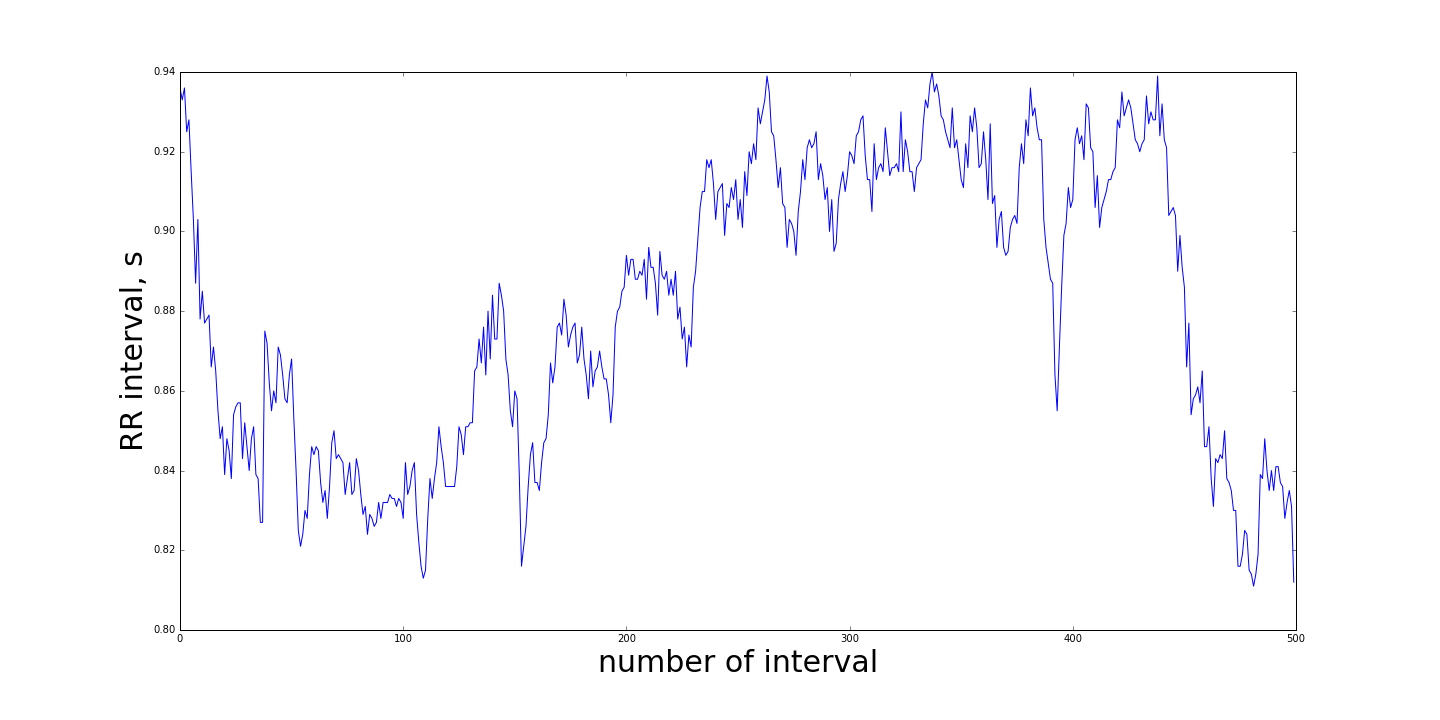
\includegraphics[width=1\linewidth]{rr_500}} c) \\
	\end{minipage}
	\hfill
	\begin{minipage}[h]{0.47\linewidth}
		\center{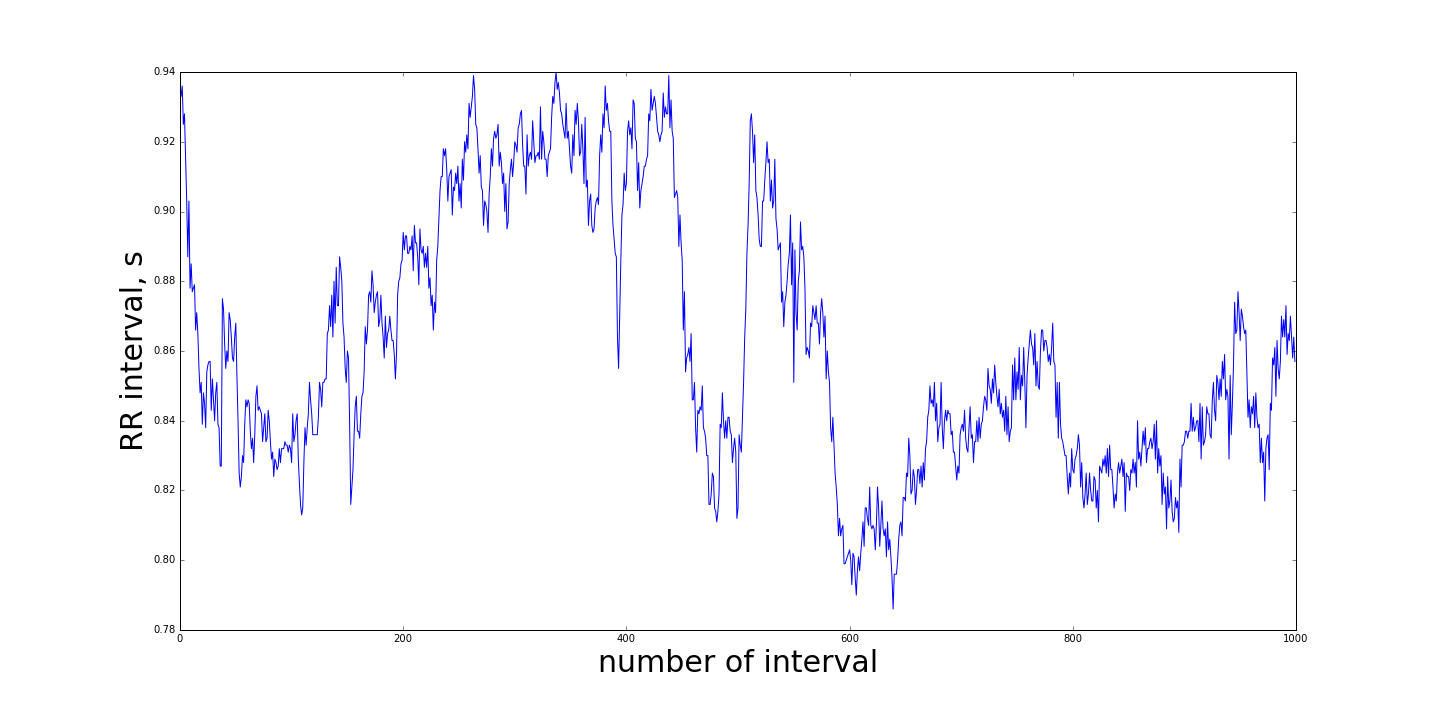
\includegraphics[width=1\linewidth]{rr_1000}} d) \\
	\end{minipage}
	\begin{minipage}[h]{0.47\linewidth}
		\center{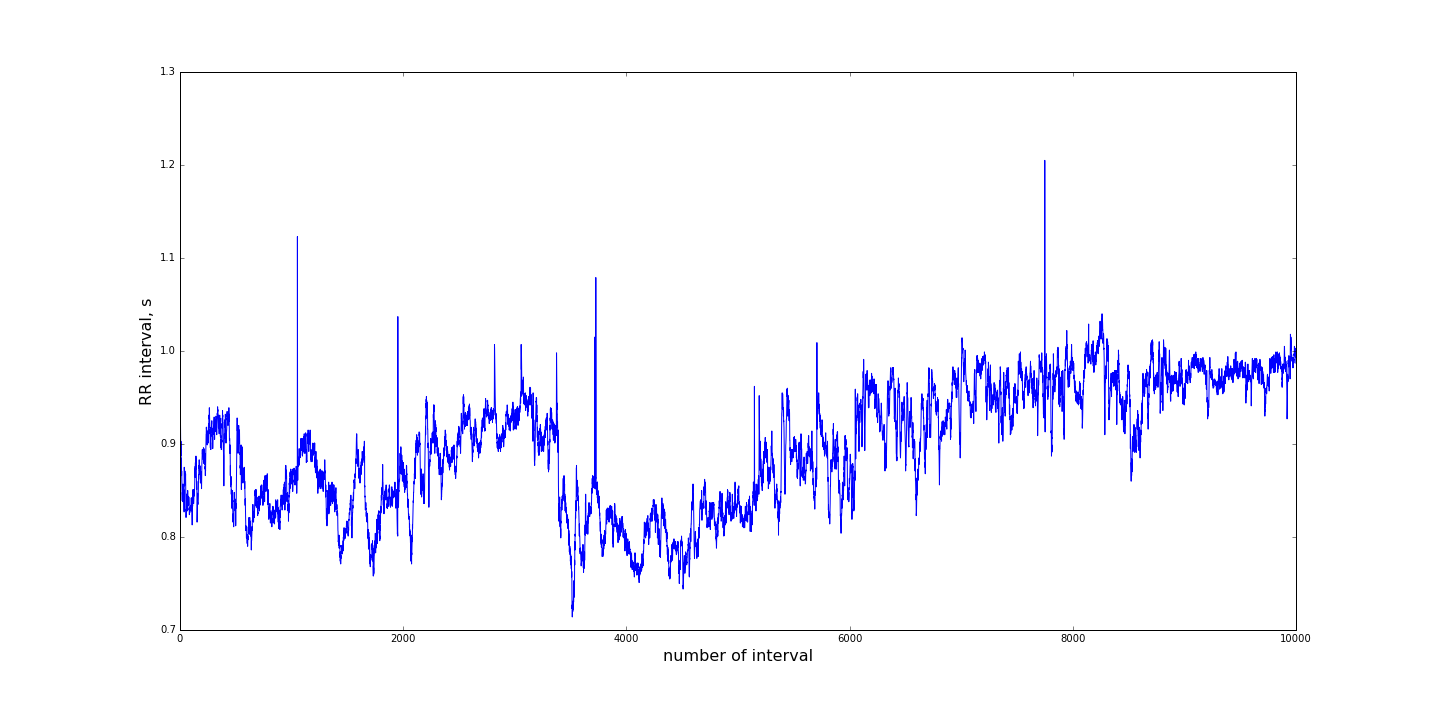
\includegraphics[width=1\linewidth]{rr_10000}} e) \\
	\end{minipage}
	\hfill
	\begin{minipage}[h]{0.47\linewidth}
		\center{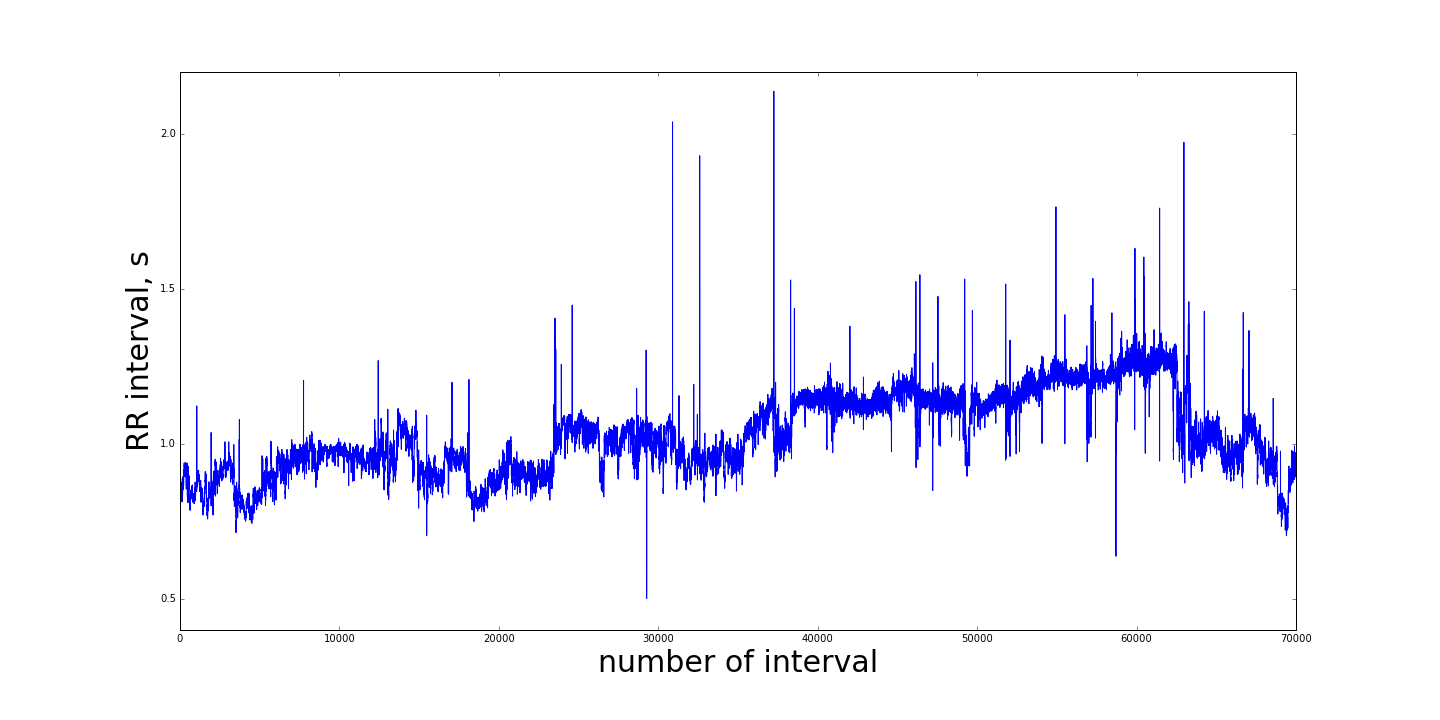
\includegraphics[width=1\linewidth]{rr_70000}} f) \\
	\end{minipage}
	\caption{RR-сигнал длительностью a)100 отсчетов $\sim$ 70с) b) 200 отсчетов
		c) 500 отсчетов d) 1000 отсчетов e)10000 отсчетов ($\sim $2 часа) f)70000 отсчетов.}
	\label{ris:real_RR}
\end{figure}


\subsection{Анализ RR сигнала}
После фильтрации ЭКГ и выделения R-пиков мы получаем последовательность RR-интервалов. В данной главе речь пойдет о работе с RR-сигналом - последовательностью промежутков времени между R-пиками (RR-интервалами).

Существует перечень стандартных признаков, которые считаются информативными и обычно используются при анализе RR-сигнала.
Их можно разделить на несколько групп.

\begin{enumerate}
	\item Признаки, основанные на подсчете стандартных статистик анализе RR интервалов. При данном анализе часто подсчитываются следующие характеристики \cite{pNN, metric_of_hrv}.
	\begin{enumerate}
		\item SDNN - стандартное отклонение интервалов от среднего, вычесленого почти всегда в течение 24 часов. SDNN отражает все циклические компоненты, ответственные за изменчивость в период записи, поэтому она представляет собой общую вариабельность.
		\item 	RMSSD ("среднеквадратичное последовательных различий») - квадратный корень из среднего значения квадратов последовательных RR-интервалов. Второй момент.
		\item SDSD ("стандартное отклонение последовательных разностей") - стандартное отклонение последовательных разностей между соседними  RR-интервалами.
		\item NN50, количество пар последовательных RR-интервалов, которые отличаются более чем 50 мс.
		\item pNN50, доля NN50 - NN50 делится на общее количество ударов (R-пиков).
		\item NN20, количество пар последовательных NN ударов, которые отличаются более чем 20 мс.
		\item pNN20, доля NN20.
		\item EBS ("оценивается цикл дыхания"), диапазон (макс-мин) в скользящем окне заданной длительности. Окна можно перемещать без перекрытия или с перекрытием. EBS часто используют при сборе данных, в качестве обратной связи в режиме реального времени.
		\item skewness - третий момент случайной велечины - в теории вероятностей и статистике, является мерой несимметричности распределения вероятностей некоторой вещественной случайной величины около ее среднего значения. Значение асимметричности может быть положительным или отрицательным, или даже неопределенным.
		\item kurtosis - это мера "tailedness" распределения вероятностей некоторой вещественной случайной величины. Это описание формы распределения, точнее насколько "хвостатым" оно является. 
	\end{enumerate}
	\item Геометрические методы \cite{geometric_metric}
	\begin{enumerate}
		\item график Пуанкаре \cite{poinkare_plot}. Он представляет собой точечную диаграмму: на оси абсцисс отложены значения текущего интервала RR, а на оси ординат – следующего по времени значения RR. Форма графика Пуанкаре категоризирована в несколько функциональных классов.
		\item фрактальные размерности \cite{fractal_dim}. Фрактальную размерность n-мерного множества можно определить с помощью формулы: $D=-\lim_{\varepsilon->0}{\frac{ln(N_\varepsilon)}{ln(\varepsilon)}}$,
		где $N_\varepsilon$ — минимальное число $n-$мерных «шаров» радиуса $\varepsilon$, необходимых для покрытия множества.
	\end{enumerate}	
	\item Частотный анализ
	
	\begin{enumerate}
		\item суммарная мощность спектра (0.003–0.6 Hz)
		\item VLF (very low frequency component) мощность самых низкочастотных компонент (0.003–0.02 Hz)
		\item LF (low-frequency component) мощность низкочастотных компонент сигнала (0.02–0.15 Hz)
		\item HF (high-frequency component) мощность высокочастотных компонент сигнала (0.15–0.6 Hz)
		\item LF/HF
	\end{enumerate}
	
	\item Подсчет кореляций следующих NN ударов от предыдущих \cite{autocorr_metric}
	\item Нелинейные методы \cite{non_linear_metric}
	
	\begin{enumerate}
		\item детрентный флуктуационный анализ \cite{fluct_analis}.
		
		\item энтропия \cite{entropy1}. Чтобы определить элементарную энтропию Шеннона выборки из $N$
		значений рассматриваемого ряда ${x}$, находим максимальную ($х_{max}$) и минимальную ($x_{min}$) величины в анализируемом ряде. Разбиваем этот интервал ($х_{max} – x_{min}$) на $n$ подинтервалов (уровней) таким образом, чтобы величина интервала $\Delta x$ была не меньше доверительного интервала данных наблюдений. 
		
		Рассматриваем выборку как «сообщение», а подынтервалы $i$ как «алфавит». Далее находим число значений выборки ${x_k}$, попавших в каждый из подинтервалов, и определяем относительную населенность уровня $p_i$ (вероятность попадания значения из выборки в подинтервал $i$, то есть относительную частоту встречаемости «буквы» в «сообщении») $p_i = \Delta N_i / N$. Очевидно, что при этом $\sum{\Delta N_i} = N$, $\sum{p_i} = p$ . Элементарная энтропия выборки определяется как энтропия Шеннона на данном наборе pi: $H = - \sum{p_i*log(p_i)}$ 
		\item и др. \cite{other_analis1, other_analis2, other_analis3}
	\end{enumerate}	
\end{enumerate}
\subsection{Неклассический частотный анализ ЭКГ}
Также существует другой метод работы с ЭКГ сигналом, описанный в работах Воронцова и Успенского \cite{voronzov}. В работе описана технология информационного анализа электрокардиосигналов. 

Сначал каждую электрокардиограммыу преобразуют в последовательность интервалов и амплитуд кардиоциклов, затем в символьную последовательность — кодограмму и, наконец, в числовой вектор — признаковое описание фиксированной размерности, что позволяет строить диагностические правила по обучающей выборке методами машинного обучения.

Эту технологию можно описать следующими шагами:
\begin{enumerate}
	\item Преобразование элетрокаргиограммы в последовательность интервалов ($R_n$), амплитуд ($T_n$), и угла их отношений ($\alpha_n=arctg(R_n/T_n)$)(рис. \ref{ris:voronzov_R_T_A})
	
	\begin{figure}[h!]
		\begin{center}
			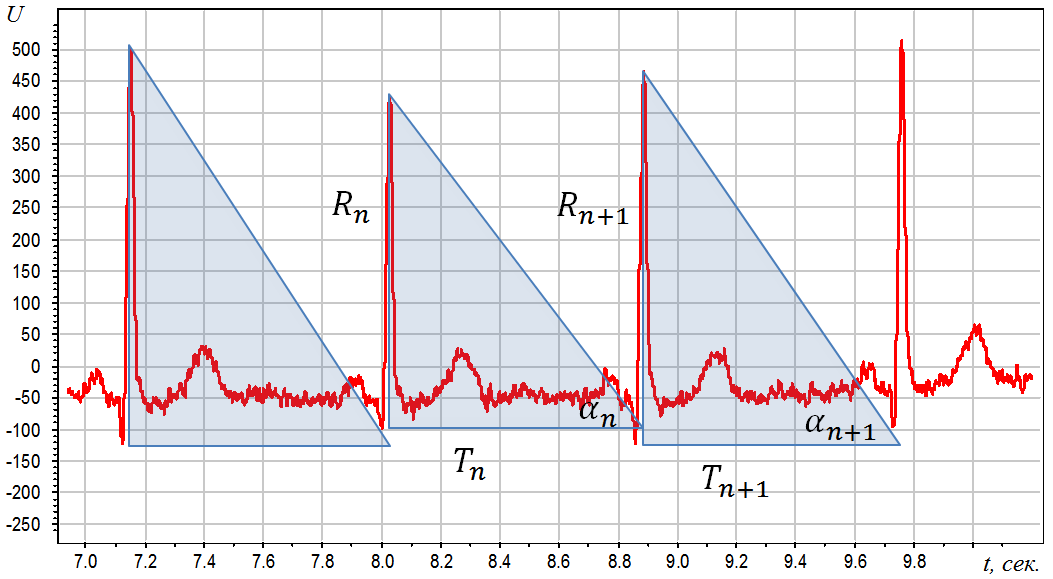
\includegraphics[scale=0.3]{voronzov_R_T_A}
			\caption{Пример электрокардиограммы.}
			\label{ris:voronzov_R_T_A}
		\end{center}
	\end{figure}
	\item Подсчет приращения этих величин. ($dR_n = R_{n+1} - R_{n}$, $dT_n = T_{n+1} - T_{n}$,$d\alpha_n = \alpha_{n+1} - \alpha_{n}$)
	\item Перевод приращений в бинарный формат ($><0$).
	\item Кодировка  всех возможных комбинаций (их 6) буквами алфавита. Это производилось по следующемо правилу:
	\begin{itemize}
		\item если $R_n<R_{n+1}$, $T_n<T_{n+1}$, $\alpha_n<\alpha_{n+1}$, то $s_n=a$
		\item если $R_n>=R_{n+1}$, $T_n>=T_{n+1}$, $\alpha_n<\alpha_{n+1}$, то $s_n=b$		
		\item если $R_n<R_{n+1}$, $T_n>=T_{n+1}$, $\alpha_n<\alpha_{n+1}$, то $s_n=c$		
		\item если $R_n>=R_{n+1}$, $T_n<T_{n+1}$, $\alpha_n>=\alpha_{n+1}$, то $s_n=d$		
		\item если $R_n<R_{n+1}$, $T_n<T_{n+1}$, $\alpha_n>=\alpha_{n+1}$, то $s_n=e$		
		\item если $R_n>=R_{n+1}$, $T_n>=T_{n+1}$, $\alpha_n>=\alpha_{n+1}$, то $s_n=f$		
	\end{itemize}
	После этих предразований ЭКГ сигнал оказывался закодирован символьной строкой $x = [s_0, s_1, ...,s_n, ..., s_N]$, кодограммой.

	\begin{figure}[h]
		\begin{center}
			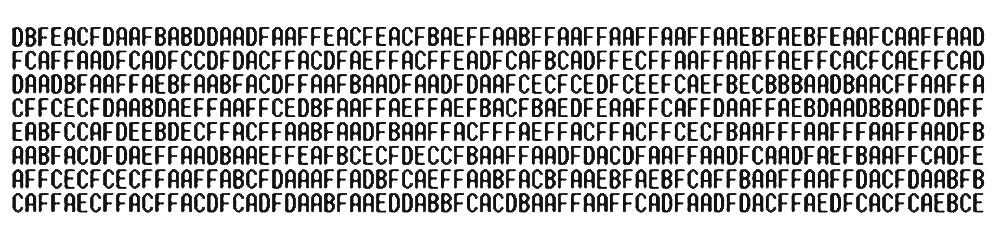
\includegraphics[scale=0.3]{voronzov_codograma}
			\caption{Пример кода}
			\label{ris:voronzov_codograma}
		\end{center}
	\end{figure}
	\item Подсчет частот всех возможных триграмм в кодограмме.
\end{enumerate}
Подсчитанные частоты являются входными данными для алгоритмов машинного обучения в данных работах. Размерность вектора признаков здесь равна 216 ($6^3$).
 
Далее исследователи проводят статистический анализ информативности каждой триграммы. Во-первых, они проверяют, что частота триграммы в исходной последовательности кардиоциклов, и в сигнале с вырезанными и перемешанными кардиоциклами отличаются. То есть проверяют, что вариации амплитуд и интервалов в соседних кардиоциклах неслучайны и зависимы. Во-вторых, что частоты триграмм в выборках больных и здоровых людей различаются.

После этого, перевзвешенные на основе информативности частоты триграм подаются на вход алгоритму классификации, который и выдает решающее правило, на основе которого будет проводится дальнейшая классификация. В качестве алгоритмов машинного обучения здесь использовались логистическая регрессия, наивный байесовский классификатор и случайный лес.

Точность классификации для различных болезней (при равных чувствительности и спецефичности) - от 56\% до 98\%.

\section{Предсказание сна}
Актуальность исследований сна и ее психологических факторов обусловлена, в первую очередь, практической необходимостью. 
Расстройства сна, такие как бессоница, которая по данным эпидемиологии встречается у 28-45\% населения, в половине случаев является важной проблемой, требующей лечения \cite{sleep3}.
При этом 1.5-3\% населения постоянно и 25-29\% эпизодически принимают снотворные препараты. 
У больных бессоницей выше риск психических и соматических заболеваний и смертность. Существующие исследования показали, что у людей, страдающих бессонницей, риск развития гипертонии на 350\% выше, чем у обычных людей. 
Бессонница также является фактором риска для сахарного диабета, тревоги и депрессии.
Среди пожилых людей до 35\% населения имеют проблемы со сном, а именно до 20\% мужчин и до 50\% женщин. \cite {sleep1, sleep2}

Для точной оценки бессоницы необходимы замеры длительности сна. Золотым стандартом для данной задачи у человека является анализ паттернов мозговых волн (ЭЭГ) впервые описаный Rechtschaffen и Калес \cite{eeg_for_sleep}. Наиболее распространенным методом анализа сна является полисомнография, которая сочетает в себе анализ ЭЭГ-записи и различных физиологических сигналов, таких как электромиография (ЭМГ), электроокулография (ЭОГ), сигналы о дыхательной деятельности, уроветь насыщения крови кислородом, электрокардиограммы (ЭКГ) и анализ видео. В полисомнографии, для каждых 30-секундных интервалов на основе этих сигналов принимается решение о состоянии человека а этот момент времени (спит/бодствует). Этот метод обычно проводится в контролируемых условиях стационара и нуждается в медицинской помощи по настройке датчиков, мониторинга и анализа. Также для этого аналази необходим эксперт по сну, и хотя он при это используются компьютерные программы, исследование является дорогостоящим и трудоемким. Трудно интегрировать датчики полисомнографии в носимые устройств, так как они довольно громоздкие, энергоемкие и очень восприимчивые к шуму. Кроме того, для записи ЭЭГ требуется много электродов, которые наклеиваются на кожу головы, что делает его очень громоздким и неудобным для пользователя. 
В добавок эти системы неудобны так для проведения замеров, нобходимо провести ночь в медицинском центре в специальных установках.

Сейчас исследуются новые методы наблюдения за сном \cite{monitor_sleep, monitor_sleep2, monitor_sleep3}. Интерес в портативных устройствах в данной сфере постоянно растет. В домашних условиях, где полисомнография обычно не доступна, врачи полагаются на актиграфию для мониторинга сна \cite{actigrafia}. В этом методе, акселеромтр крепится на конечность (обычно на запястье). Недостатком данного метода является неверная классификация периодов низкой активности, которая классифицируются как сон после автономной компьютерной обработки. Для актиграфия предложены много различных алгоритмов классификации, но часто они не могут справиться с проблемой неверной классификации элементарных задач, как чтение и просмотр телевизионных передач. В последнее время, будильники, использующие акселерометры были коммерциализированы.

Изменения активности вегетативной нервной системы (ВНС) во время переходов - сон/пробуждение были успешно идентифицированы в качестве надежного источника информации \cite{tosleep}. Изменения в работе ВНС отражаются в различных физиологических сигналах, таких как частота сердечных сокращений, артериальное давление, проводимость кожи и т. д. 

Относительно текущей точности предсказания сна по ЭКГ сигналу человека можно привести следующие информацию.

В статье \cite{sleep_accuracy_3} 2009 разрабатывается метод классификации на сон/бодроствование. Данные для исследования -  записи с 6 здоровых испытуемых мужского пола в возрасте от 23 до 29 лет. ЭКГ и информация о дыхании были записаны с помощью системы Heally. Были собраны записи длительностью минимум 16 часов  (минимум 6 часов до сна, период сна, время после сна). Записей было 18. Для каждых 10 секунд было известно, когда человек спал (разметка проводилась людьми по видео и дополнительным датчикам,надеваемым на ночь). Средняя точность предсказаний только с использованием ЭКГ сигнала - 72\%.

В работе \cite{sleep_accuracy_2} 2016 года анализируются сигналы ЭКГ, собраные при помощи смартфона на основе пульсоксиметра, одновременно со стандартной процедурой полисомнографии для 160 детей в детской больнице Британской Колумбии. Были размечены периоды сна/бодрствования на протяжении всего исследования. Производительность данной модели на полном наборе тестов показали среднию точность 77\%, чувствительность 80\%, и специфичность 70\%.

\section{Алгоритмы машинного обучения}
\subsection{Случайный лес}

Случайный лес \cite{random_forest} в настоящее время считается одним из самых эффективных алгоритмов машинного обучения. Он представляет собой ансамбль решающих деревьев, каждое из которых строится по случайным подвыборкам, полученным в результате сэмплирований с возвращениями объектов обучающей выборки.

Кроме того, при создании очередного узла каждого дерева выбор признака, на основе которого происходит разбиение, производится не из всего множества признаков, а из их случайного подмножества. Классификация объектов проводится путем простого голосования: каждое решающее дерево относит объект к одному из классов, решение принимается на основании большинства голосов. Для оценки качества построенного классификатора удобно ввести дискриминантную функцию, оценивающую степень принадлежности объекта к классу, например, равную доле деревьев, голосующих за этот класс.

Пусть $C_m$ — множество деревьев в ансамбле, построенном по обучающей выборке; $g_{c_m}(S)$ — класс, к которому дерево $c_m \in C_m$ относит объект $S$. Тогда решающее правило представляется в виде:
$a_m(S) = b_m(S) > \beta_m$, $b_m(S) = \frac{1}{|C_m|}*\sum_{c_m \in C_m}[g_{c_m}(S) = 1]$,

где $b_m(S)$ — доля деревьев, относящих прецедент $S$ к классу 1 (дискриминантная функция); $\beta_m$ — порог принятия решения (равен 1/2 при простом голосовании деревьев).

\subsection{Рекуррентные нейронные сети}
Рекуррентная нейронная сеть – один из типов нейронных сетей \cite{neural_network}, в котором присутствует обратная связь. Другими словами в выход более позднего слоя сети поступает на вход более слоя, считающегося ранее.
\begin{figure}[h]
	\begin{center}
		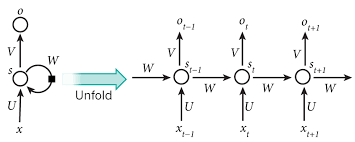
\includegraphics[scale=1]{rnn_shem}
		\caption{Рекуррентная нейронная сеть}
		\label{ris:rnn_shem}
	\end{center}
\end{figure}


Рекуррентные нейронные сети имеют ряд преимуществ перед обычными.
\begin{itemize}
	\item Разнообразные виды входных данных
	\item Способность строить неявные модели данных
	\item Устойчивость к выбросам
\end{itemize}

Рекуррентные сети применяются в таких задачах как:
\begin{itemize}
	\item распознавание устной и письменной речи \cite{rnn_for_speech_recognition, rnn_for_text_recognition};
	\item машинный перевод \cite{rnn_for_translation};
	\item предсказания временных рядов \cite{rnn_for_prediction};
	\item создание описаний для изображений.
\end{itemize}

Основной проблемой при использовании рекуррентных нейронных сетей является проблема исчезающего градиента (vanishing gradient problem \cite{vanishing_gradient_problem}). Если честно подсчитывать градиент на каждой итерации обучения, он будет выражаться через произведение градиентов, подсчитанных на всех предыдущих итерация. Если градиенты были малы – наш градиент будет просто не заметен и обучение встанет надолго. 

Проблема исчезающего градиента была подробно рассмотрена Хохрейтером и Шмидхубером, которые разработали LTSM архитектуру \cite{create_lstm}, которая устойчива к данной проблеме. Данная архитектура оказалась проста в использовании и стала стандартным средством борьбы с исчезающим градиентом. Также были осуществлены попытки других способов решения данной проблемы:
\begin{itemize}
	\item обратное распостранение во времени (Backpropagation through time) \cite{Backpropagation}. Используется для обучения сетей Элмана.
	\item использование мощного вторичного алгоритма оптимизации \cite{rnnlearning1}
	\item регуляризация весов в RNN, что гарантирует, что градиент не обращается в нуль \cite{rnnlearning2}
	\item отказ от обучения текущих весов и очень
	осторожная инициализация параметров RNN \cite{rnnlearning3}.
\end{itemize}
	
Также была обнаружена проблема сильного возрастание градиента, но она легко решилась наложением ограничений на модуль градиента.

\subsubsection{LSTM}

Данный слой успешно борется с проблеммай исчезающего градиента. Каждый нейрон в данном слое представняет собой "ячейку памяти" (рис. \ref{ris:ltsm}). Данные ячейки организованны для хранения информации и позволяют более качествеено обрабатывать длинные входные последовательности.

\begin{figure}[h]
\begin{center}
	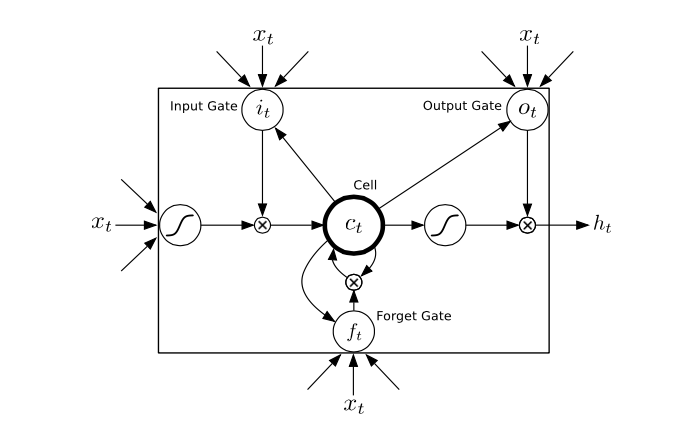
\includegraphics[scale=0.36]{ltsm.png}
	\caption{LSTM ячейка}
	\label{ris:ltsm}
\end{center}
\end{figure}


Пускай на вход LSTM ячейке памяти подается часть входной последовательности $x_t = (x_1, ..., x_N)$ и предыдущие выходной вектор признаков $h_{t-1} = (h_1, ..., h_M)$. Ячейка должна подсчитать вектор признаков $h_t$. Ячейка организованны следующим обрахом:


\begin{equation}
	i_i = \sigma(W_{xi}*x_t+W_{hi}*h_{t-1}+W_{ci}*c_{t-1}+b_i)
\end{equation}
\begin{equation}
	f_t = \sigma(W_{xf}*x_t+W_{hf}*h_{t-1}+W_{cf}*c_{t-1}+b_f)
\end{equation}
\begin{equation}
	c_t = f_t*c_{t-1}+i_t*\tanh(W_{xc}*x_{t-1}+W_{hc}*h_{t-1}+b_c)
\end{equation}
\begin{equation}
	o_t = \sigma(W_{xo}*x_t+W_{ho}*h_{t-1}+W_{co}*c_t+b_o)
\end{equation}
\begin{equation}
	h_t = o_t*\tanh(c_t)
\end{equation}

Здесь $\sigma = \frac{1}{1+e^{-x}} $ - сигмоида, логистическая функция, принимающая значения от 0 до 1. А i, f, o и c - вход ячейки, клетка памяти, выход ячейки и клетка активации, по содержимому которой решается, будет ли использоваться ектор из клетки памяти. Все вышеперечисленные вектора имеют размерность $h_t$.

